%%%%%%%%%%%%%%%%%%%%%%%%%%%%%%%%%%%%%%%%%%%%%%%%%%%%%%%%%%%%%%%%%%%%%%%%%%%%%%%%
%characterization.tex: Chapter on ground characterization measurements:
%%%%%%%%%%%%%%%%%%%%%%%%%%%%%%%%%%%%%%%%%%%%%%%%%%%%%%%%%%%%%%%%%%%%%%%%%%%%%%%%
\chapter{Detector Characterization}
\label{characterization_chapter}
%%%%%%%%%%%%%%%%%%%%%%%%%%%%%%%%%%%%%%%%%%%%%%%%%%%%%%%%%%%%%%%%%%%%%%%%%%%%%%%%

There were more than four dozen detector wafers fabricated and characterized for \ac{EBEX}. 
The characterization measurements provided here are only for those wafers which flew in the \ac{EBEX2013} flight. 
The measurements were performed in testbeds designed to be as similar to the final flight configuration as possible. 
The three testbeds used were: a dedicated \ac{EBEX} test cryostat at the University of Minnesota, a test cryostat at McGill University, and the \ac{EBEX} cryostat itself, made dark. 
In each of these cryostats, the wafer was mounted and coupled to the readout electronics as was done for flight. 
We cooled the wafers to 250-320~mK, where the exact temperature depended on the testbed. 
%highlight the difference between the light and dark configuration (and that you were attempting to minimize such that they were tested under conditions as similar to operation as possible.


%%%%%%%%%%%%%%%%%%%%%%%%%%%%%%%%%%%%%%%%%%%%%%%%%%%%%%%%%%%%%%%%%%%%%%%%%%%%%%%%
% Parameter Measurements {{{
%%%%%%%%%%%%%%%%%%%%%%%%%%%%%%%%%%%%%%%%%%%%%%%%%%%%%%%%%%%%%%%%%%%%%%%%%%%%%%%%
\section{Detector Parameter Measurements}
\label{sec:parameter_measurements}
%%%%%%%%%%%%%%%%%%%%%%%%%%%%%%%%%%%%%%%%%%%%%%%%%%%%%%%%%%%%%%%%%%%%%%%%%%%%%%%%

We measured detector parameters with the goals of controlling fabrication and predicting the sensitivity the detectors would be able to achieve. 

%%%%%%%%%%%%%%%%%%%%%%%%%%%%%%%%%%%%%%%%%%%%%%%%%%%%%%%%%%%%%%%%%%%%%%%%%%%%%%%%
\subsection{Normal Resistance}
\label{sec:normal_resistance}
%TOWARDS NORMAL RESISTANCES
%%%%%%%%%%%%%%%%%%%%%%%%%%%%%%%%%%%%%%%%%%%%%%%%%%%%%%%%%%%%%%%%%%%%%%%%%%%%%%%%

\begin{figure}[htbp]
\begin{center}
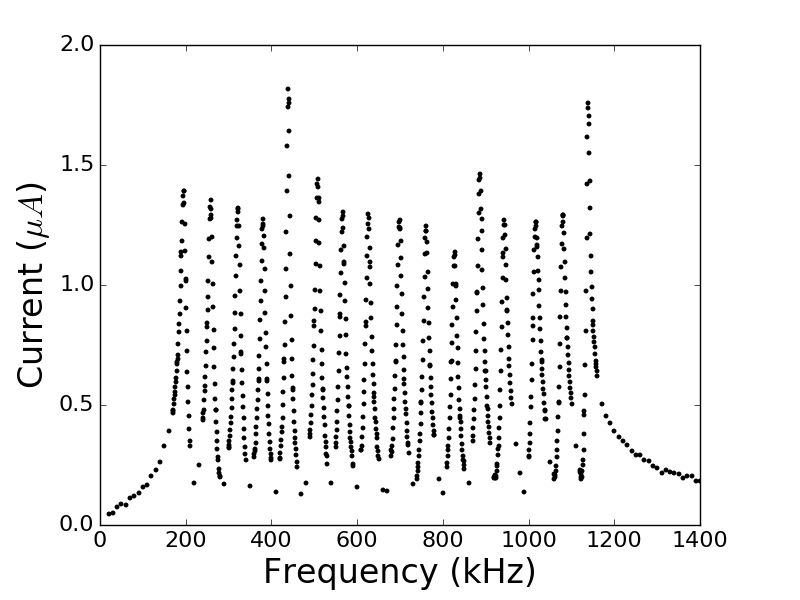
\includegraphics[width=0.48\textwidth]{figures/netanal_b16_SqCh1_5K_20111005_all.png}
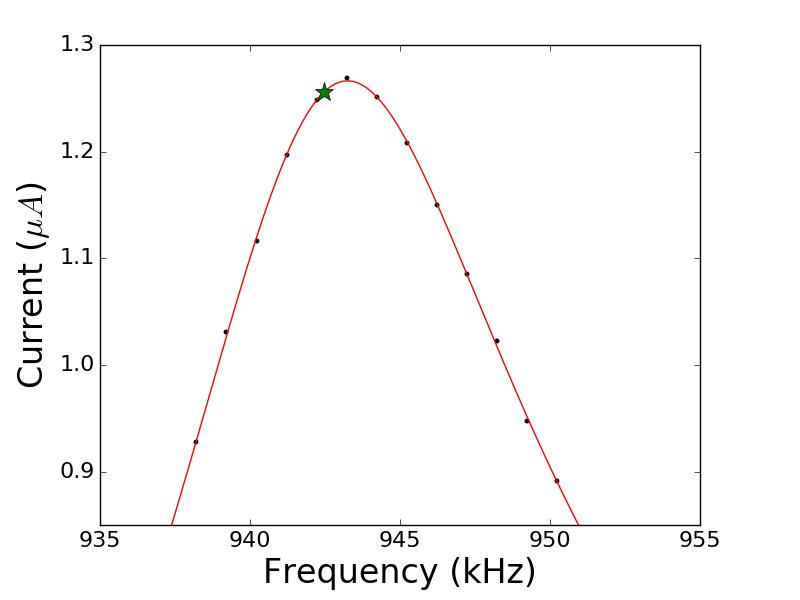
\includegraphics[width=0.48\textwidth]{figures/netanal_zoom_b16_SqCh1_5K_20111005.png}
\caption{PUT YOUR OWN FIGURE HERE. Left: an example network analysis taken during testing.
Right: a zoom on one peak (black dots) with the fitted response (red) and the optimal bias frequency (green star) minimizing crosstalk.}
\label{fig:network_analysis}
\end{center}
\end{figure}

Figure~\ref{fig:network_analysis} is a network analysis for a single comb of 16 detectors. 
The network analysis swept a voltage across the comb in frequency and measured the current response of the circuit. 
At each LC resonant frequency, the multiplexed RLC circuit peaked in current. 
Around 800~mK, when the niobium leads and aluminum wirebonds were superconducting, fitting the peak width provided the normal resistance of the \ac{TES}. 
The shape of the peak was modeled as a Lorentzian, 
\begin{equation}
Lorentzian
\end{equation}
The network analysis comb was modeled to have an impedance of 
\begin{equation}
Z_{RLC} = ???
\end{equation}
In addition to providing the resonant frequencies, the fit to this model gave the stray resistance and inductance in series with the comb. 
Typical stray resistance was about XXX $\Omega$ and typical stray inductance was XXX $uH$.
Note, the center of the current peak and the optimal frequency bias are not perfectly aligned because we wanted to maximize the current through the bolometer rather than maximize the current through the entire circuit (which included the stray resistance and inductance).

Histograms summarizing the measured normal resistance values for the three \ac{EBEX} frequency bands are shown in Fig.~\ref{fig:rn_histograms}. 
%Section~\ref{sec:detector_optimization}. the optimization section doesn't actually provide the detail I want it to provide.
The median normal resistance, $R_{normal}$, for the 150, 250, and 410~GHz bands was 1.9, 1.5, and 1.0~$\Omega$ respectively. 
The 150 and 410~GHz bimodal distributions were due to detector parameters being closely grouped within a single fabrication run, but varying between fabrication runs. 
The measured value of $R_{n}$ for the 250~GHz band closely matched the design (see 
Table~\ref{tab:Design_Params}). 
For the other two frequency bands, one mode of the distribution closely matched while the other mode was higher (lower) than design for the 150 (410)~GHz band. 
The 150~GHz detectors with a measured $R_{n}$ of 2~$\Omega$, instead of the nominal 1.5~$\Omega$, were calculated to have increased electrical cross-talk from a value of 0.5\% to 0.9\% and decreased loopgain by 30\%. 
The 410~GHz detectors with a measured $R_{n}$ of 1~$\Omega$, two-thirds of the design value, were calculated to have increased Johnson noise by 20\% relative to the nominal expected value of 4.0 pA$/\sqrt{\mathrm{Hz}}$ (9.4~aW$/\sqrt{\mathrm{Hz}}$); see Equation~\ref{eqn:noisebudget}.


%The consequences of overshooting this value, as is the case for many of the 150~GHz detectors, are an increase in the detector voltage bias leakage, which is proportional to $R^2$ \citep{dobbs_revSciInst_2012}, and a decrease in the loopgain, which is inversely proportional to R. 
%% if R is higher, then johnson current noise is decreased since it goes like 1/sqrt(R)
%% if R is higher, then stability requirement has R/(2*pi*L) > 5.8/tau_tes is more satisfied
%For a detector dropped to 85\% in the transition, having a normal resistance of 1.9~$\Omega$ instead of 1.5~$\Omega$ results in a bias leakage increase of 60\%, increasing the cross-talk from 0.5\% to 0.8\%, and a loopgain decrease of 30\%. 
%The consequence of undershooting the normal resistance, as is the case for many of the detectors on wafer 410-28, is an increase in the Johnson current noise. The Johnson noise is proportional to $1/\sqrt{R}$, so that noise term increases by 20\% given a value of 1.0~$\Omega$ instead of 1.5~$\Omega$.



%\comred{Assume detector optimization explains what about the electronics set our target to be 1.5~$\Omega$? Ben says "The requirement is really ~1.25 because what actually matters is Rtes in transition for the L/R requirement.  So depending on how deep we get in to the transition we could start anywhere just above 1.2 Ohms to operate at 0.88 to 1.0 Ohms." BUT. When determining which Rfrac to tune to, we didn't do this calculation. Rather, we noted, in general, below 80\% $R_{start}$, we had (not well understood) excess noise and so opted to go to 85\%. What I'm trying to say is, in practice, the operating fracRn value was not chosen carefully on a bolo by bolo basis or even a wafer by wafer basis to achieve a specific L/R. Explain the consequence of having a higher or lower normal resistance, e.g. 150s and one of the 410s (was it the 410 that operated or the 410 that was saturated?)? Ben says "Increased johnson noise and possibly bolo stability.  However, I'm not sure if either of these effects were detected in the wafers in test cryostats, Palestine, or flight."}


\begin{figure}[ht!]
\centering
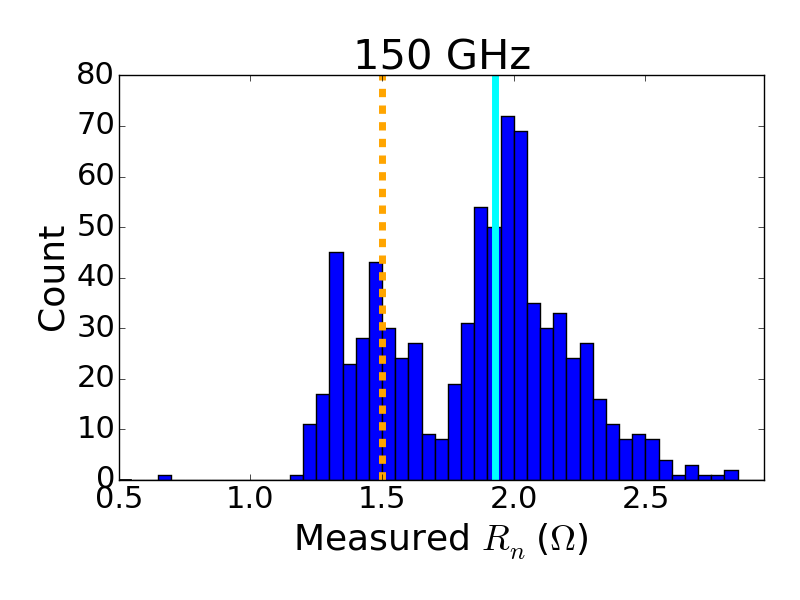
\includegraphics[width=0.31\textwidth]{figures/150_rn_hist.png}
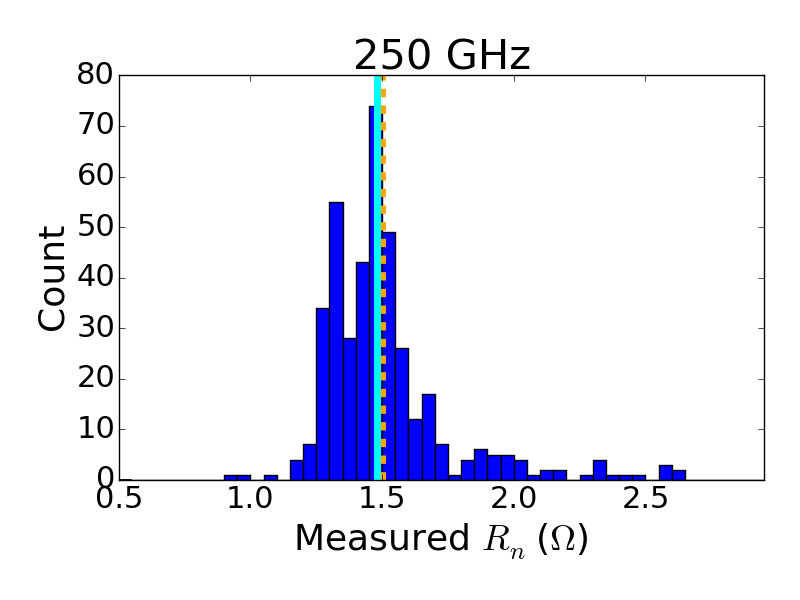
\includegraphics[width=0.31\textwidth]{figures/250_rn_hist.png}
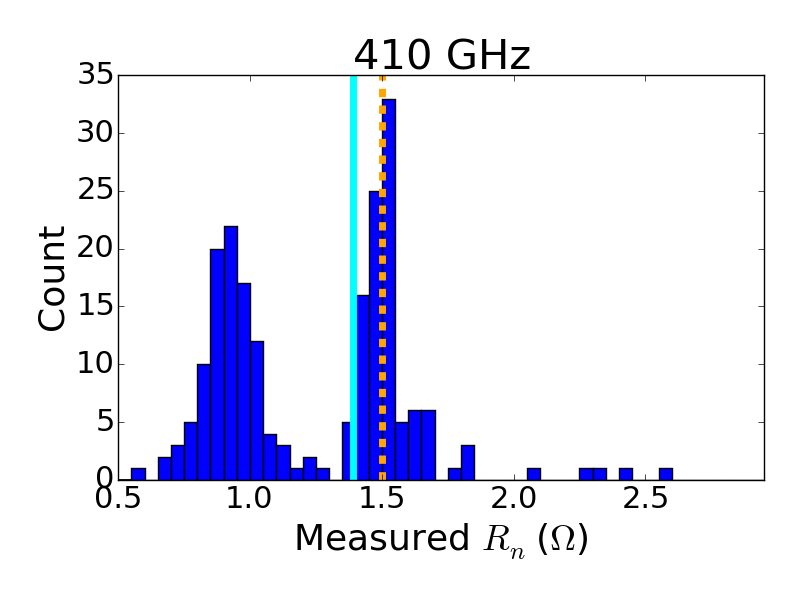
\includegraphics[width=0.31\textwidth]{figures/410_rn_hist.png}
\caption{Histogram of measured normal resistances $R_{n}$ for each of the frequency bands, including the median (vertical cyan)  
and design (vertical gold dashed) values.
}
\label{fig:rn_histograms}
\end{figure}

%%%%%%%%%%%%%%%%%%%%%%%%%%%%%%%%%%%%%%%%%%%%%%%%%%%%%%%%%%%%%%%%%%%%%%%%%%%%%%%%
\subsection{Critical Temperature}
\label{sec:critical_temp}
%TOWARDS CRITICAL TEMPERATURES
%%%%%%%%%%%%%%%%%%%%%%%%%%%%%%%%%%%%%%%%%%%%%%%%%%%%%%%%%%%%%%%%%%%%%%%%%%%%%%%%

\begin{figure}[ht!]
\centering
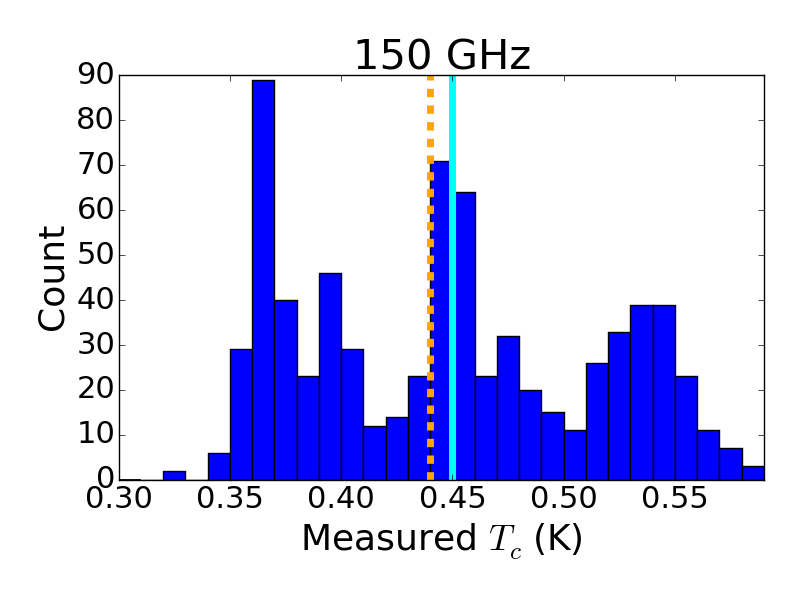
\includegraphics[width=0.31\textwidth]{figures/150_tc_hist.png}
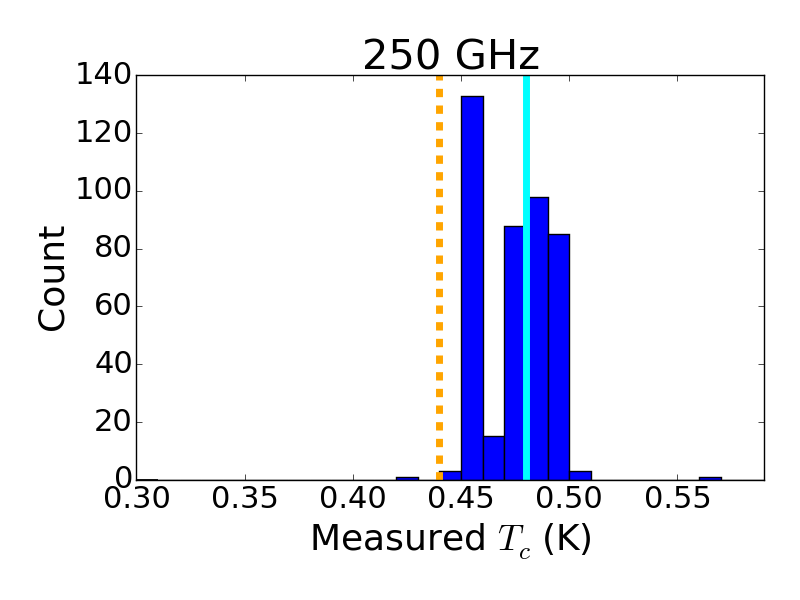
\includegraphics[width=0.31\textwidth]{figures/250_tc_hist.png}
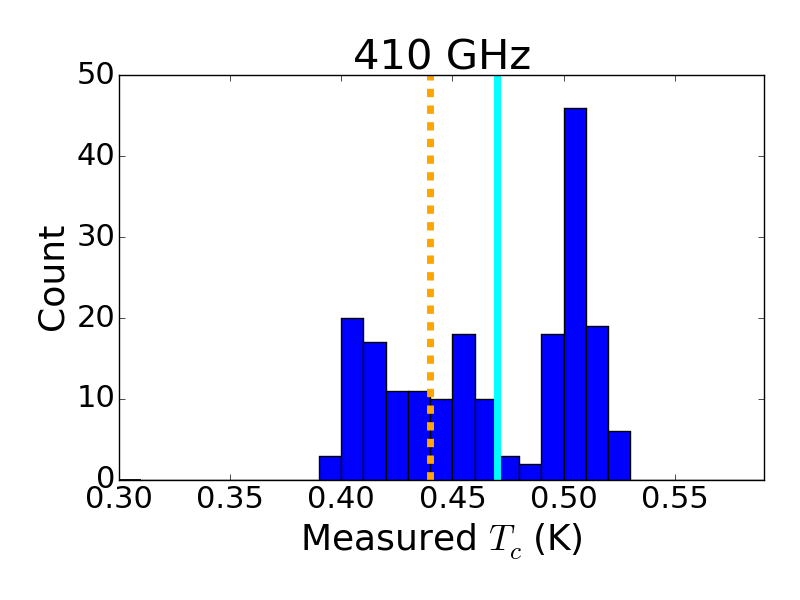
\includegraphics[width=0.31\textwidth]{figures/410_tc_hist.png}
\caption{Histogram of measured critical temperature values for the detectors in each frequency band including the median (vertical cyan) and design (vertical gold dashed) values. 
\label{fig:tc_histograms} }
\end{figure}

%%%%%%%%%%%%%%%%%%%%%%%%%%%%%%%%%%%%%%%%%%%%%%%%%%%%%%%%%%%%%%%%%%%%%%%%%%%%%%%%
\subsection{Thermal Conductance}
\label{sec:thermal_conductance}
%TOWARDS THERMAL CONDUCTANCES 
%%%%%%%%%%%%%%%%%%%%%%%%%%%%%%%%%%%%%%%%%%%%%%%%%%%%%%%%%%%%%%%%%%%%%%%%%%%%%%%%

\begin{figure}[ht!]
\centering
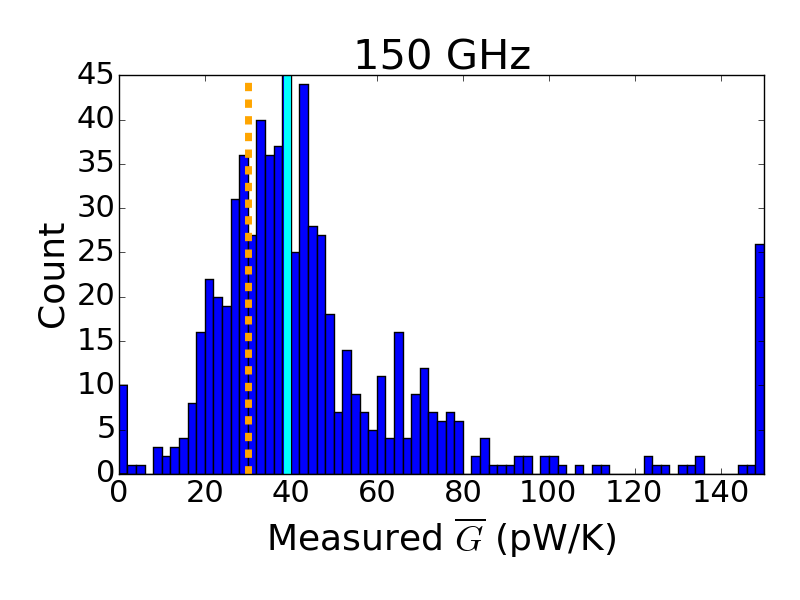
\includegraphics[width=0.31\columnwidth]{figures/150_g_bar_hist.png}
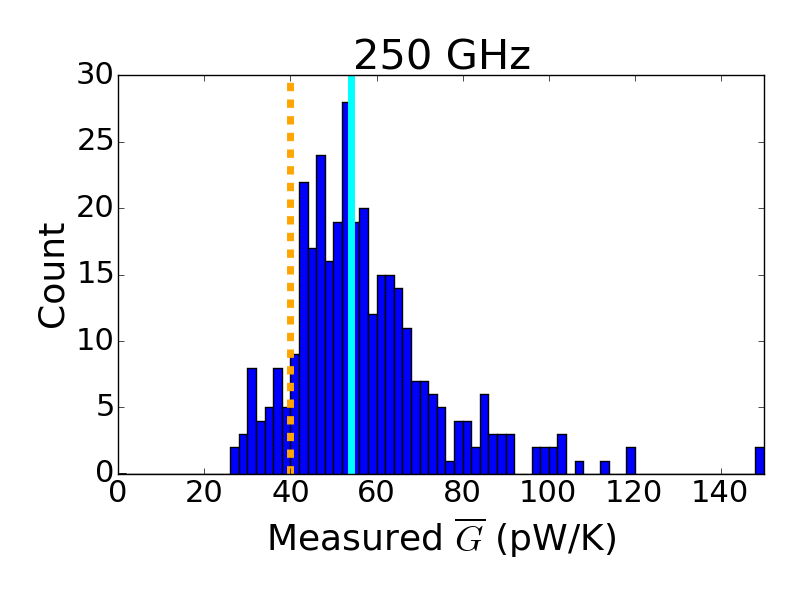
\includegraphics[width=0.31\columnwidth]{figures/250_g_bar_hist.png}
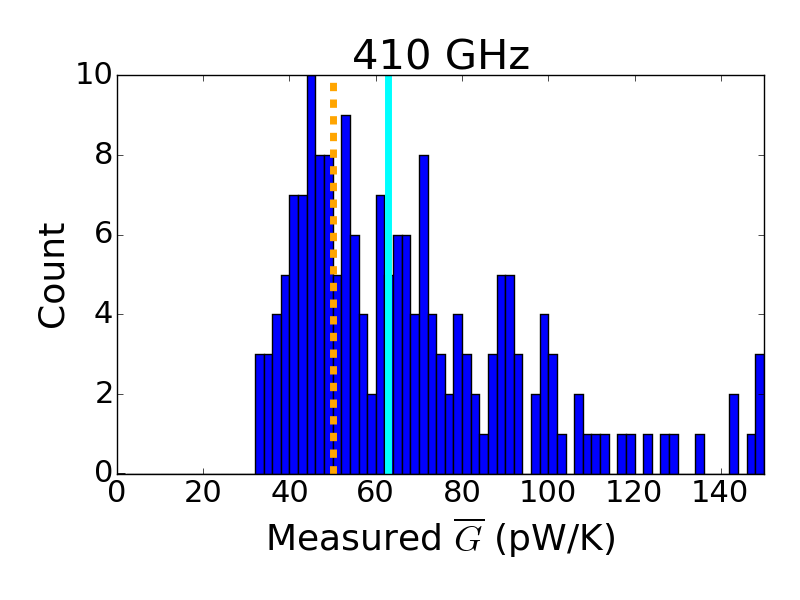
\includegraphics[width=0.31\columnwidth]{figures/410_g_bar_hist.png}
\caption{Histograms of the measured average thermal conductance values for the three frequency bands including the 
median (vertical cyan) and design (vertical gold dashed) values. 
We piled measurements of  $\overline{G}$ exceeding 150~pW/K into the last histogram bin.
}
\label{fig:G_Histograms} 
\end{figure}


%%%%%%%%%%%%%%%%%%%%%%%%%%%%%%%%%%%%%%%%%%%%%%%%%%%%%%%%%%%%%%%%%%%%%%%%%%%%%%%%
\subsection{Optical Efficiency}
\label{sec:optical_efficiency}
%%%%%%%%%%%%%%%%%%%%%%%%%%%%%%%%%%%%%%%%%%%%%%%%%%%%%%%%%%%%%%%%%%%%%%%%%%%%%%%%

\begin{figure}[ht!]
\begin{center}
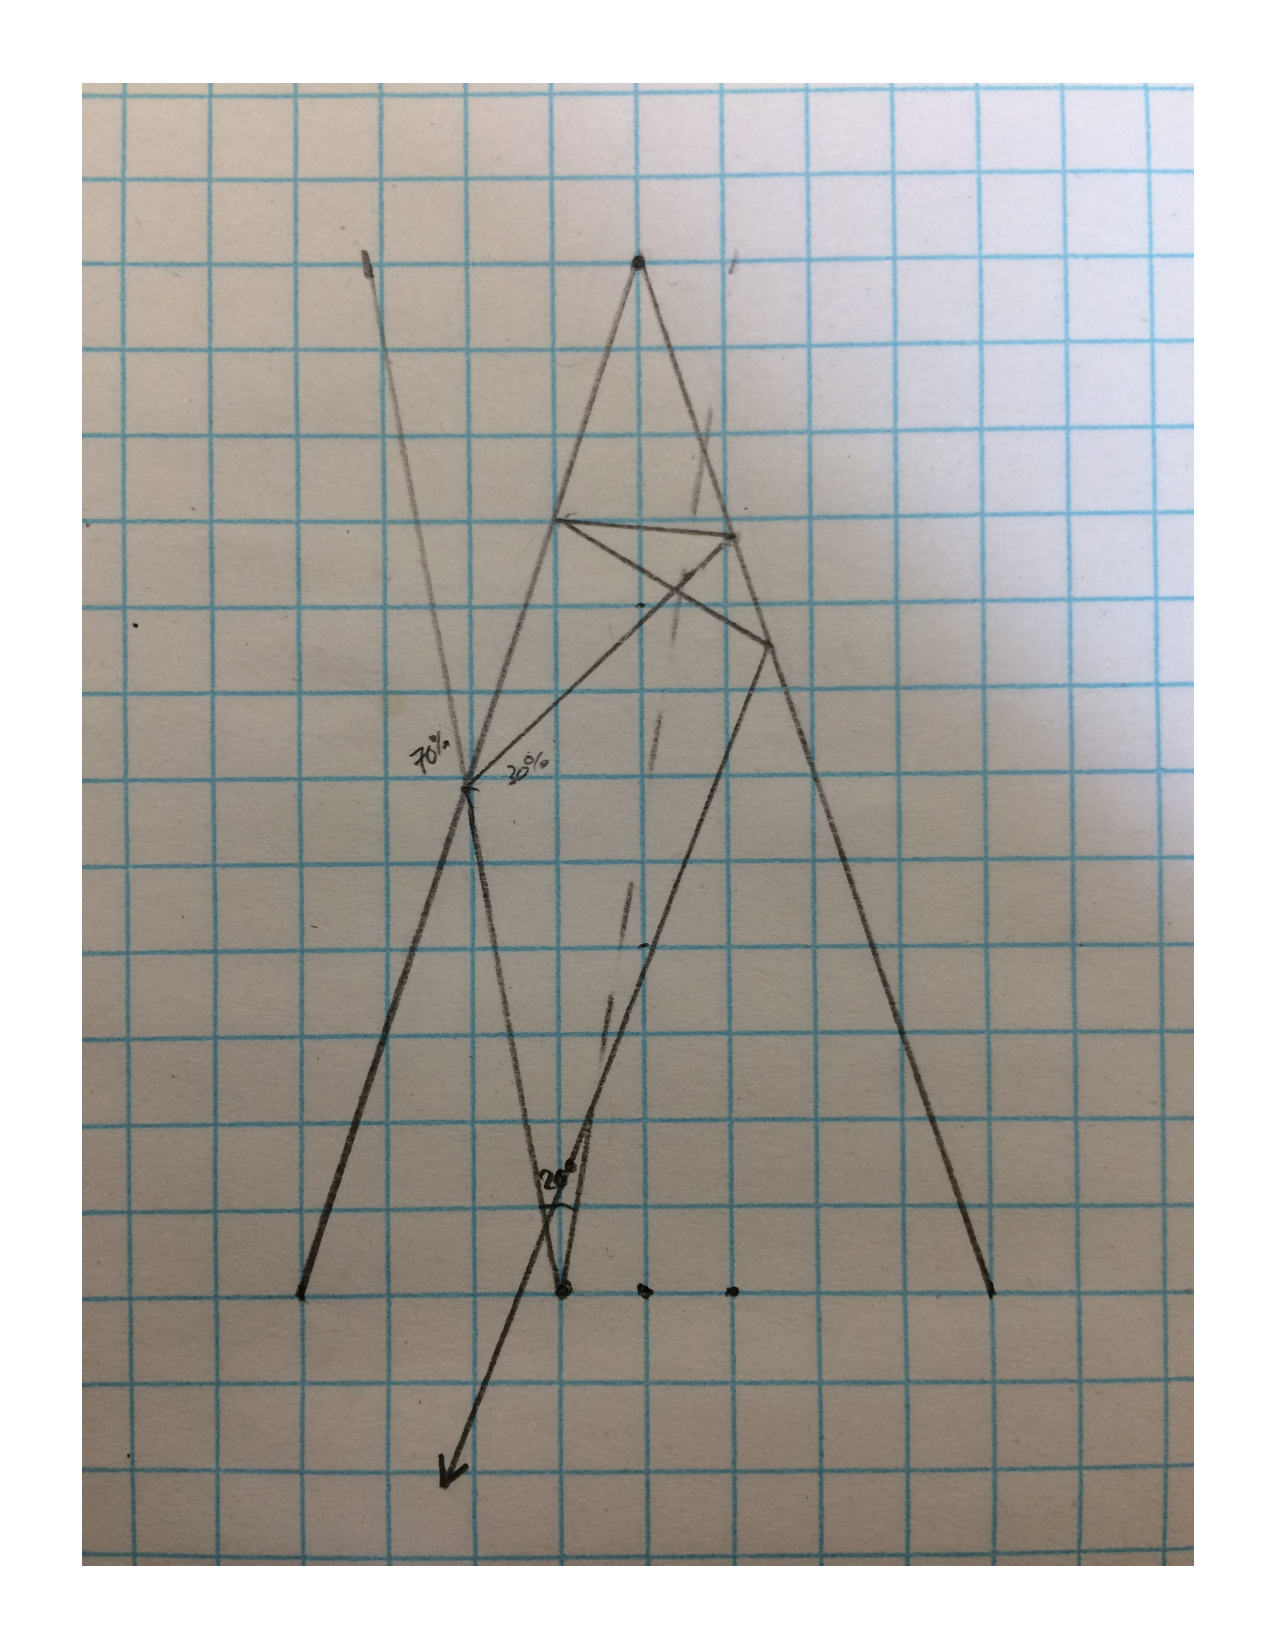
\includegraphics[height=2.5in]{figures/blackbody_design2}
\caption{Eccosorb blackbody design. 
\label{fig:blackbody_design} }
\end{center}
\end{figure}

\begin{figure}[ht!]
\begin{center}
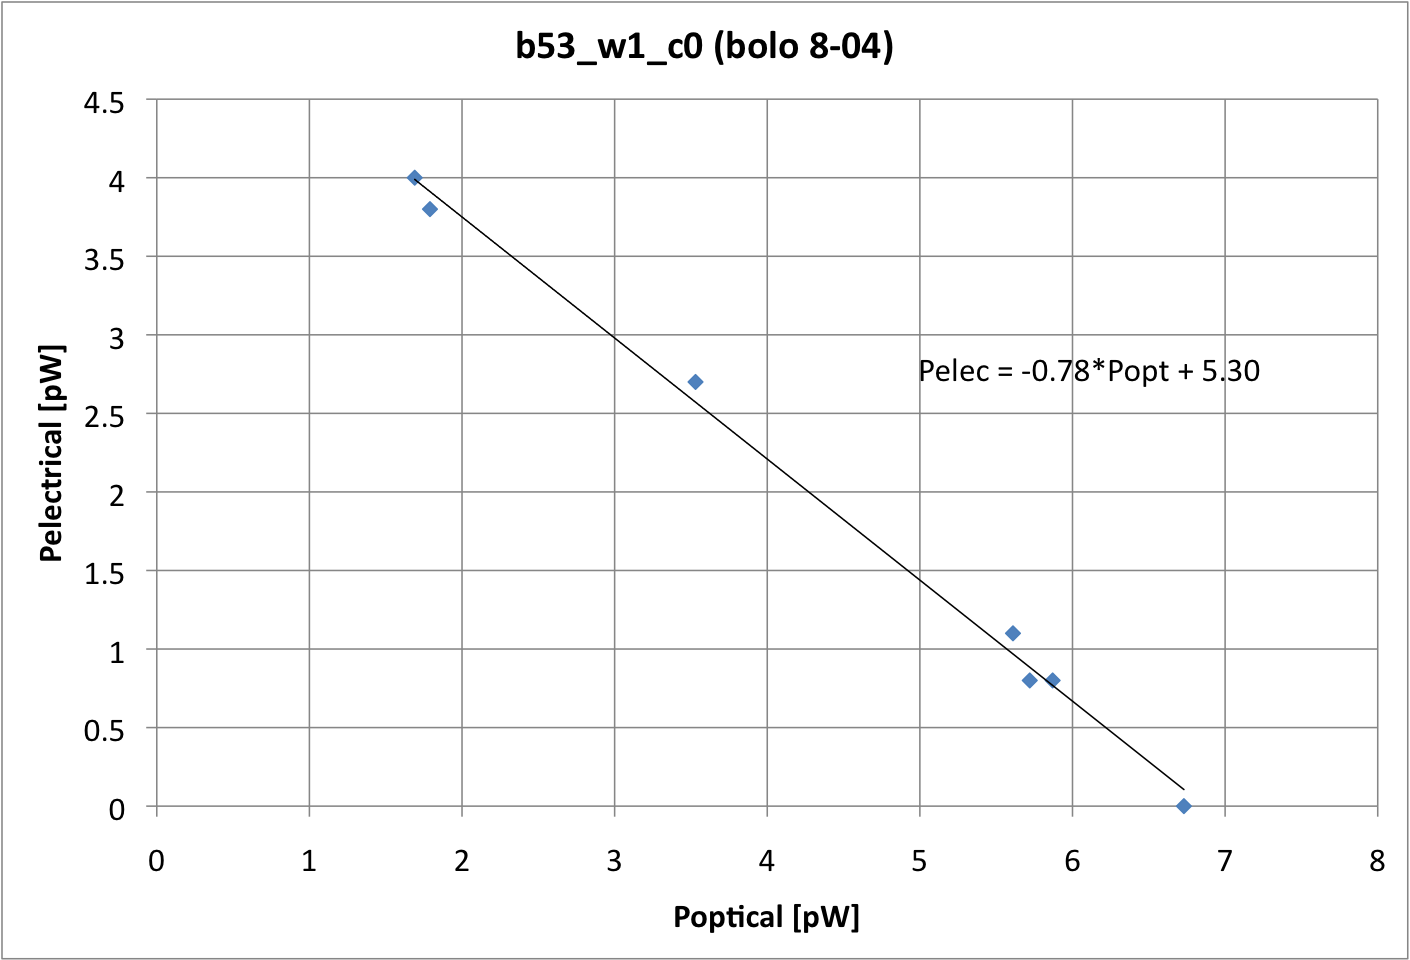
\includegraphics[height=2.5in]{figures/Nb01_PelecvsPopt_b53_w1_c0}
\caption{One 150-01 detector electrical power as function of blackbody power. The slope is the detector's optical efficiency. 
\label{fig:pelec_vs_popt} }
\end{center}
\end{figure}


\begin{figure}[ht!]
\begin{center}
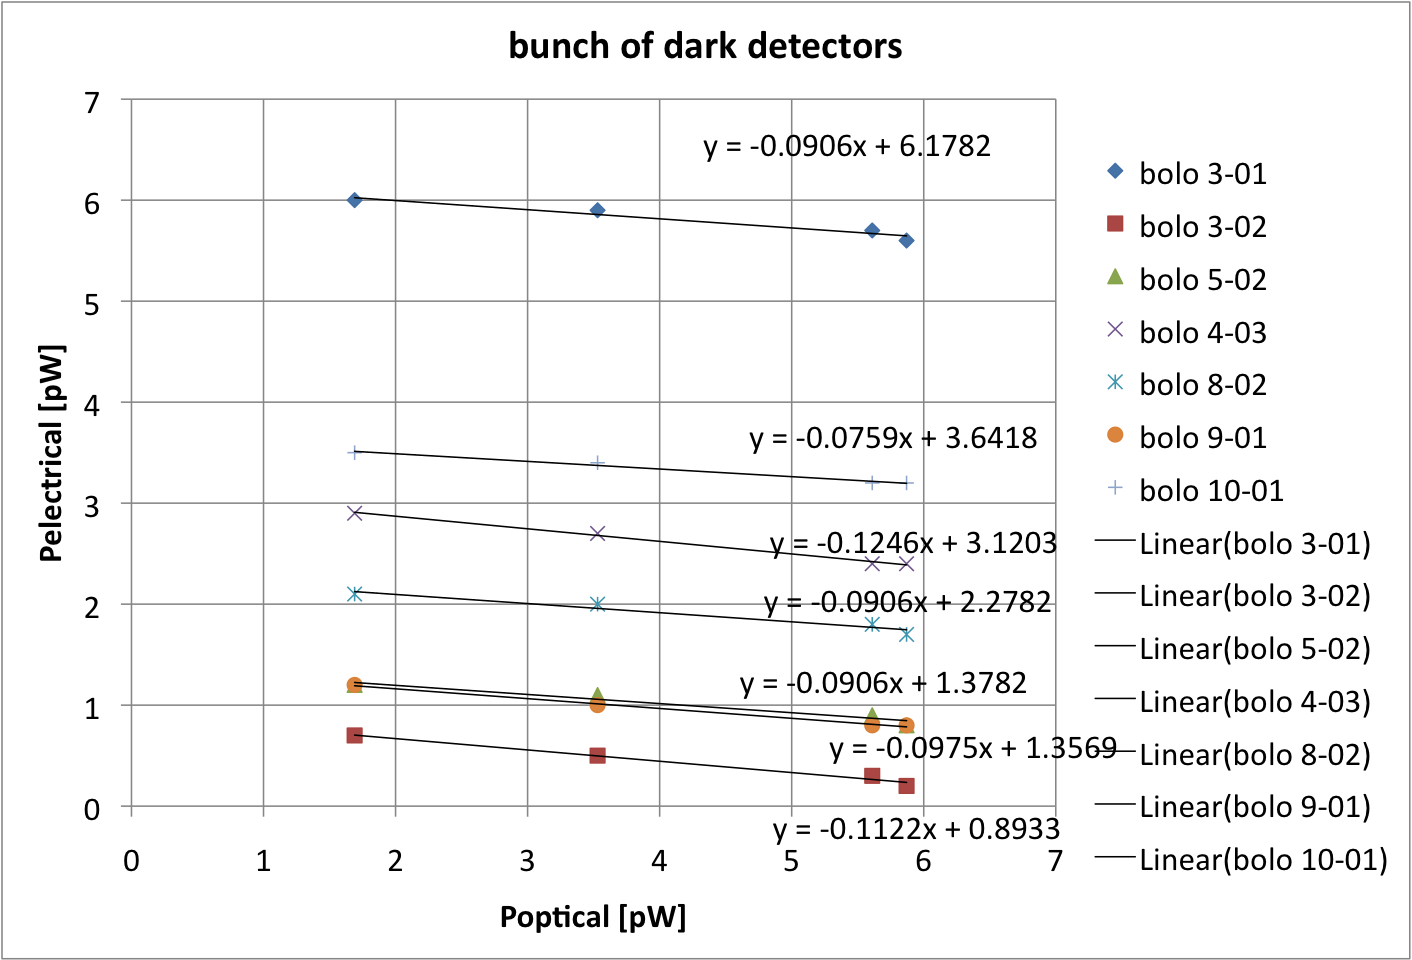
\includegraphics[height=2.5in]{figures/darkdetectoreffs}
\caption{The dark detectors also observed a decrease in electrical power needed to keep the detector in the transition as the black body temperature was turned up. The slope of this line gives the "efficiency" of the dark detectors. Some measure of the level of optical cross talk?
\label{fig:dark_optical_efficiencies} }
\end{center}
\end{figure}


%%%%%%%%%%%%%%%%%%%%%%%%%%%%%%%%%%%%%%%%%%%%%%%%%%%%%%%%%%%%%%%%%%%%%%%%%%%%%}}}


%%%%%%%%%%%%%%%%%%%%%%%%%%%%%%%%%%%%%%%%%%%%%%%%%%%%%%%%%%%%%%%%%%%%%%%%%%%%%%%%
% Dark Noise Performance {{{
%%%%%%%%%%%%%%%%%%%%%%%%%%%%%%%%%%%%%%%%%%%%%%%%%%%%%%%%%%%%%%%%%%%%%%%%%%%%%%%%
\section{Dark Noise Performance}
\label{sec:dark_nosie}
%%%%%%%%%%%%%%%%%%%%%%%%%%%%%%%%%%%%%%%%%%%%%%%%%%%%%%%%%%%%%%%%%%%%%%%%%%%%%%%%


\begin{figure}[ht!]
\begin{center}
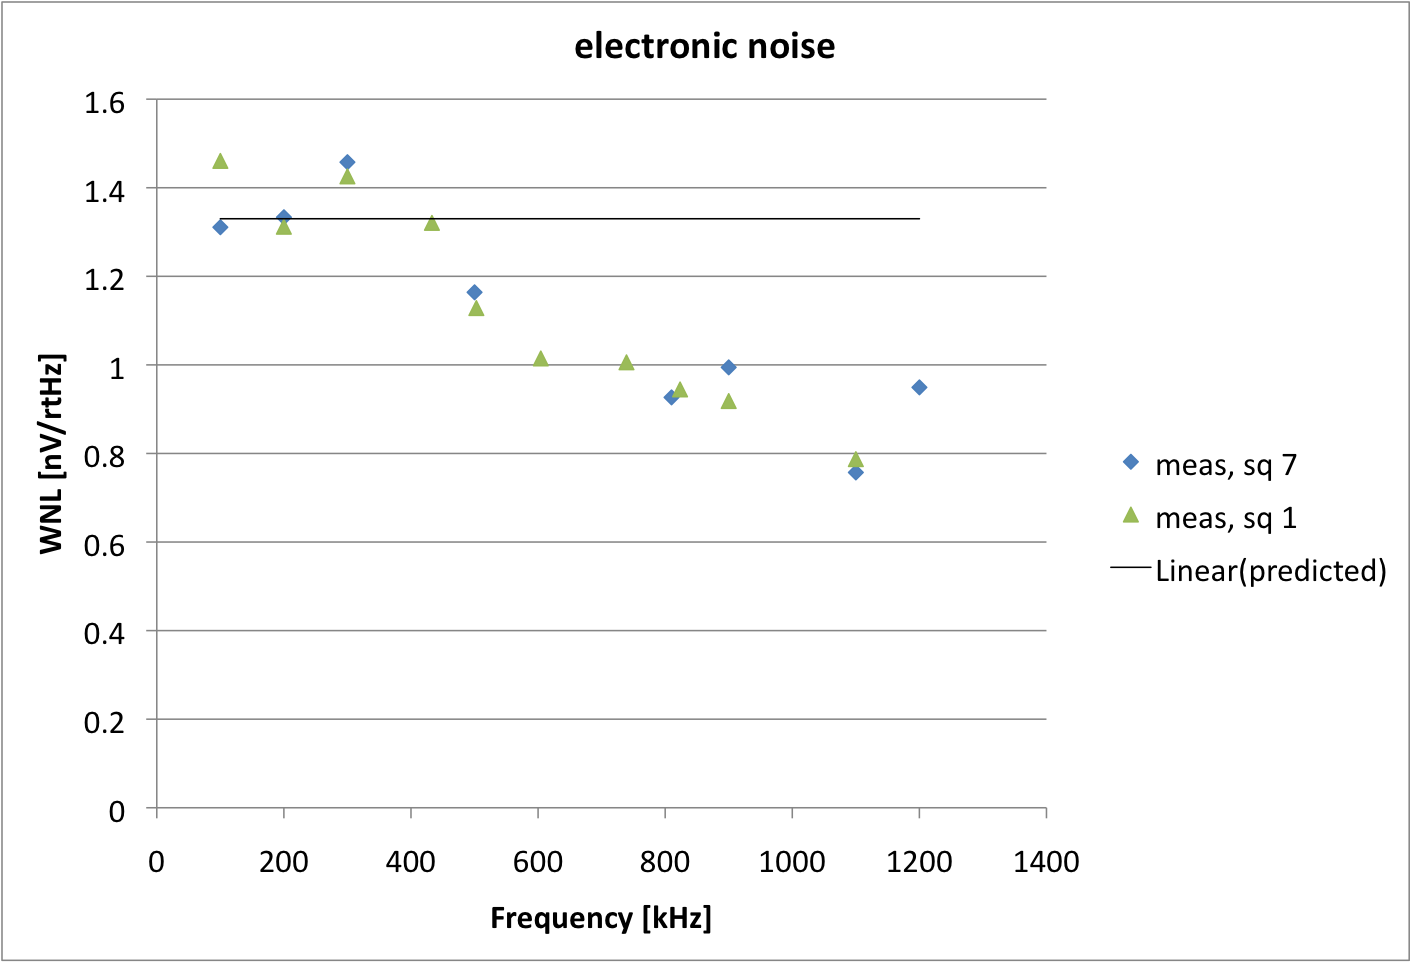
\includegraphics[height=2.5in]{figures/electronic_noise_sq1_sq7}
\caption{Electronic noise of warm electronics in \ac{ETC}. Units of $nV/\sqrt{Hz}$. This is probing the system from point A to point B. It includes the noise of ... .
\label{fig:dark_electronic_noise} }
\end{center}
\end{figure}

\begin{figure}[ht!]
\begin{center}
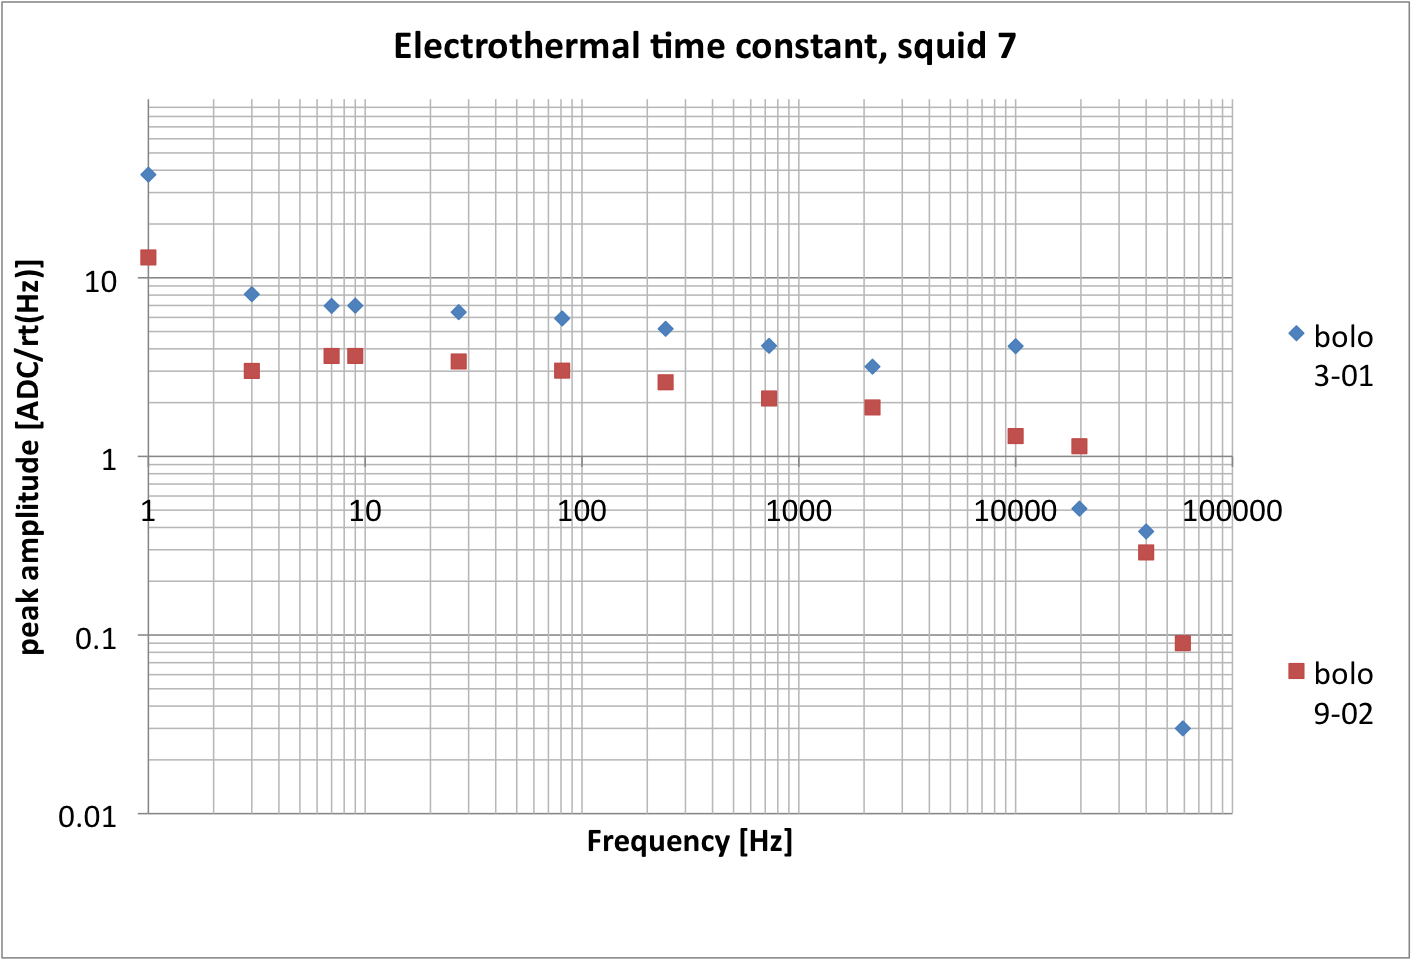
\includegraphics[height=2.5in]{figures/Nb01_squid7_etau_morepts}
\caption{Electrothermal time constants of two bolometers on 150-01. What does the fit to this data give? This is the time constant between the TES and the web? As expected, the for the web to thermalize is much faster than the optical time constant (time for light to couple to the web). 
\label{fig:electrothermal_tau} }
\end{center}
\end{figure}

\begin{figure}[ht!]
\begin{center}
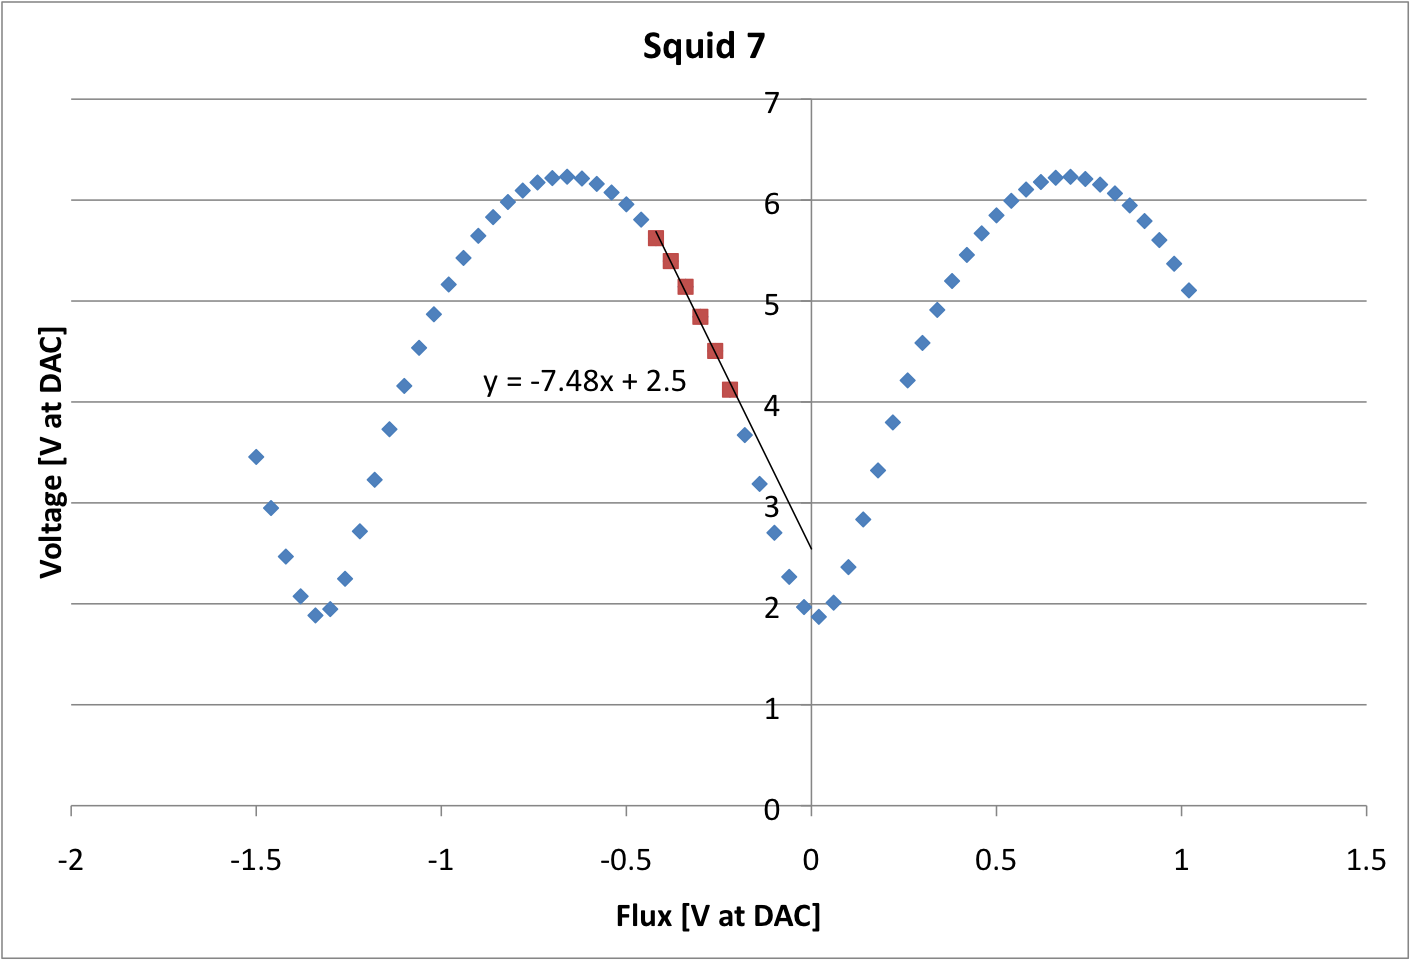
\includegraphics[height=2.5in]{figures/squid7_transimp}
\caption{\ac{SQUID} voltage versus current/flux curve. Operating regime is highlighted. Transimpedance, $dV/d\phi$ is the slope of the line.
\label{fig:squid_transimpedance} }
\end{center}
\end{figure}

\begin{figure}[ht!]
\begin{center}
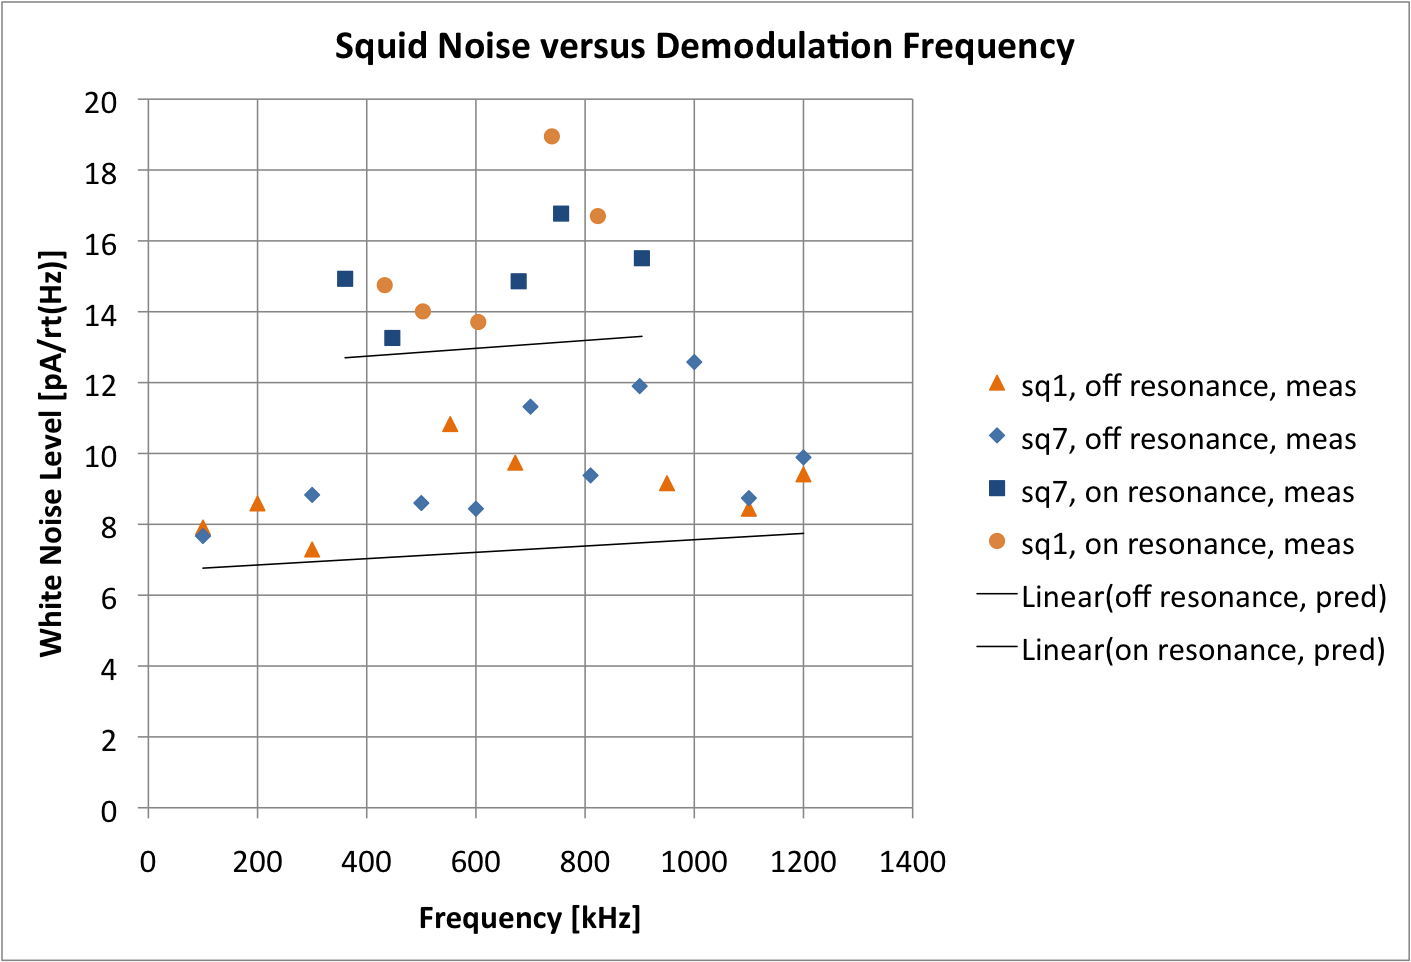
\includegraphics[height=2.5in]{figures/squidnoise_temp}
\caption{\ac{SQUID} noise in \ac{ETC} as function of demodulation frequency. At detector demodulation frequencies, the Johnson noise term of the bolometer roughly doubles the noise.
\label{fig:dark_squid_noise} }
\end{center}
\end{figure}



%%%%%%%%%%%%%%%%%%%%%%%%%%%%%%%%%%%%%%%%%%%%%%%%%%%%%%%%%%%%%%%%%%%%%%%%%%%%%}}}
